
\section*{Revisjonshistorie}
\begin{center}
 \begin{tabular}{|p{1.5cm} p{5.5cm}|} 
 \hline
 År & Forfatter \\ [0.5ex] 
 \hline\hline
 2020 & Kolbjørn Austreng  \\ 
 \hline
 2021 & Kiet Tuan Hoang \\
 \hline
 2022 & Kiet Tuan Hoang \\
 \hline
  2023 & Kiet Tuan Hoang \\
 \hline
 2024 & Terje Haugland Jacobsson\\
 & Tord Natlandsmyr \\
 \hline
\end{tabular}
\end{center}

\begin{alphasection}
\section{Introduksjon - Praktisk rundt filene}

I denne øvingen får dere utlevert en \verb|.c|-fil i \verb|source|-mappen. Tabellen under lister opp filen som kommer med i \verb|source|-mappen samt litt informasjon om dere skal endre på filen eller om dere skal la den bli i løpet av øvingen.

\begin{center}
 \begin{tabular}{|p{8.5cm} p{5.5cm}|} 
 \hline
 \textbf{Filer} & \textbf{Skal denne filen endres?}  \\ [0.5ex] 
 \hline\hline
  \verb|source/main.c| & ja  \\ 
 \hline
\end{tabular}
\end{center}

\section{Introduksjon - Praktisk rundt øvingen}
Denne øvingen er ment som en rask innføring i Linux, slik  at resten av labopplegget fremover ikke foregår i et helt ukjent miljø. Seksjon \ref{sec:2-innføring} gir en kjapp innføring i grunnleggende kommandoer som er nyttige i Linux, og som trengs for å fullføre oppgavene som følger etter i seksjon \ref{sec:3-oppgave}. Dere får godkjent øving 1 ved at dere demonstrerer foran en studass at dere har gjort alle oppgavene i seksjon \ref{sec:3-oppgave}. 
I tillegg har tre appendikser blitt lagt til (se appendiks \ref{4-appendix}, \ref{app:cygwin} og \ref{app:VM}) i tilfelle det er noen som enten har lyst til å installere Linux på egen maskin med dual booting, eller jobbe på et Unix-liknende omgivelse for Windows med Cygwin, eller installere Linux på en VM (\textbf{V}irtual \textbf{M}achine).



\section{Litt om GNU/Linux}

Linux (Linux kernel) ble først utviklet av Linus Torvalds på 90-tallet da han studerte ved Universitetet ved Helsinki. Linus ble interessert i utvikling operativsystemer gjennom sine studier, men ble frustrert av datidens lisensbegrensninger på tilgjengelige operativsystemer. I 1991 begynte han å utvikle kjernen (kernel) til det som skulle bli til Linux-kjernen som vi kjenner det i dag. En operativsystemkjerne fungerer som et bindeledd mellom maskinvare og programmer. Den er ansvarlig for å starte systemet og tildele ressurser til programmer. En kjerne er i seg selv ikke særlig nyttig uten resten av operativsystemet, slik som enhetsdrivere, brukerprogrammer, kompilatorer, osv. Heldigvis eksisterte allerede GNU prosjektet, som hadde veldig like mål om å tilby fri (som i frihet)\footnote{"Free as in freedom, not as in beer" - Richard Stallman, Grunnlegger av GNU Prosjektet} programvare, og i grunn bare manglet en velfungerende kjerne. Ved å kombinere Linux-kjernen med GNU-programvare ble Linux om til et fullverdig operativsystem som mange i dag omtaler som "GNU/Linux". 

GNU/Linux kommer i dag som flere ulike varianter, eller distribusjoner, avhengig av hvilken programvare som brukes. Noen av de mest populære distribusjonene er Debian, Fedora Linux, Arch Linux. Datamaskinene dere skal bruke på lab bruker Ubuntu, som er en variant av Debian med et mer begynnervennlig brukergensesnitt.

Et av kjerneprinsippene til både GNU- og Linux-prosjektet er at programvare, samt tilhørende kildekode, skal være åpent tilgjengelig og respektere brukerens friheter til å bruke, endre og (re)distriburere den. Dette gjelder også utviklingen av Linux. Hvem som helst kan bidra til Linux-kjernen, og kun et fåtall utviklere jobber med å vedlikeholde prosjektet profesjonelt. Projektenes dugnadsånd har vært en stor faktor i GNU/Linux sin utvikling, og holdningen har spredd seg til å bli en hjørnestein i kulturen til dagens programvareutviklere. Dette er også en av flere grunner til at programvareutviklere foretrekker å bruke Linux både til daglibruk og profesjonelt. GNU/Linux brukes i dag av Android, ChromeOS, majoriteten av tjenere på internett og stor andel av alle tilpassede datasystemer. SpaceX sin Falcon 9, NASA sin Perserverence og Tesla sine biler er bare noen få nevneverdige Linux-brukere. 



\section{Introduksjon - Grunnleggende kommandoer}\label{sec:2-innføring}

Denne seksjonen dekker stort sett det som kreves for å bruke Linux i de kommende øvingene/labene. Ubuntu er varianten/distribusjonen som er installert på Sanntidssalen, men alle kommandoene i denne seksjonen gjelder for enhver distribusjon av Linux-baserte operativsystemer. 

Ubuntu har i likhet med Windows et grafisk grensesnitt, men det er stort sett raskere å bruke en terminal når bruken er kjent. Man kan åpne terminalen ved å trykke \verb|Ctrl + Alt + T| på tastaturet, eller ved å åpne \textit{Dash} (øverst til venstre) og søke etter \verb|terminal|. 

Terminalen åpner seg i hjemmemappen, og prompten ser slik ut (avhengig av hvem som har gjort endringer på maskinen før, kan den være annerledes):



\begin{lstlisting}[mathescape=true]
student@Ubuntu:$\smallsim$$\verb|$|$\end{lstlisting}

Tildesymbolet ($\smallsim$) forteller brukeren at man er i hjemmemappen, og \verb|$| forteller at man er en vanlig bruker - i motsetning til \textit{root} som er en allmektig bruker (symboliseres med \verb|#|).

\cprotect\subsection{\lstinline{pwd}}
Første kommando som kan være lurt å vite om er \verb|pwd|. \verb|pwd| brukes for å få en oversikt over hvilken mappe man befinner seg i. Om man kaller \verb|pwd| på sanntidssalen, burde man få noe som ligner på dette: 

\begin{lstlisting}[mathescape=true]
student@Ubuntu:$\smallsim$$\verb|$|$ pwd

/home/student
\end{lstlisting}



\cprotect\subsection{\lstinline{ls}}

Videre, for å vise innholdet i mappen man befinner seg i kan man bruke kommandoen \verb|ls|. Om man kaller \verb|ls| fra hjemmemappen vil man typisk se disse mappene:

\begin{lstlisting}[mathescape=true]
student@Ubuntu:$\smallsim$$\verb|$|$ ls

Documents Downloads Pictures Music
Public Videos Desktop Templates
\end{lstlisting}


Dette er de samme mappene som kan ses i Ubuntu sin filutforsker (åpnes ved å trykke ikonet til venstre, eller ved å søke \verb|nautilus| i \textit{dash}). I tillegg kan man inspisere innholdet i en spesifikk mappe ved å kalle \verb|ls mappenavn|.

Typisk med kommandoer i Linux er at man kan legge til flagg i kommandoene for å endre oppførselen til kommandoen. Et flagg som er nyttig for \verb|ls| er \verb|-l|. Ved bruk av \verb|-l|, listes det opp hvilke typer filer som befinner seg i mappen, hvem som har brukerrettigheter, hvem som eier filene, filstørrelse, sist modifikasjonsdato, og navn. For eksempel:

\newpage

\begin{lstlisting}[mathescape=true]
student@Ubuntu:$\smallsim$$\verb|$|$ ls -l

total 48
drwxr-xr-x 2 student student 4096 Nov 18 01:49 Documents
drwxr-xr-x 2 student student 4096 Nov 18 01:49 Downloads
drwxr-xr-x 2 student student 4096 Nov 18 01:49 Pictures
drwxr-xr-x 2 student student 4096 Nov 18 01:49 Music
drwxr-xr-x 2 student student 4096 Nov 18 01:49 Public
drwxr-xr-x 2 student student 4096 Nov 18 01:49 Videos
drwxr-xr-x 2 student student 4096 Nov 18 01:49 Desktop
drwxr-xr-x 2 student student 4096 Nov 18 01:49 Templates
\end{lstlisting}

Formatet som \verb|ls -l| produserer, er illustrert i figur \ref{fig:2-flagg-ls}. Den første bokstaven (\verb|d|) betyr at filen er en mappe\footnote{I Linux er mapper også betraktet som filer.}. Deretter følger noen bokstaver som forteller hvem som har rettighetene til å endre filen. En \verb|r| betyr at man har leserettigheter, en \verb|w| betyr at man har skriverettigheter, og en \verb|x| betyr at man kan kjøre filen.

\begin{figure}[ht]
    \centering
    

\tikzset{every picture/.style={line width=0.75pt}} %set default line width to 0.75pt        

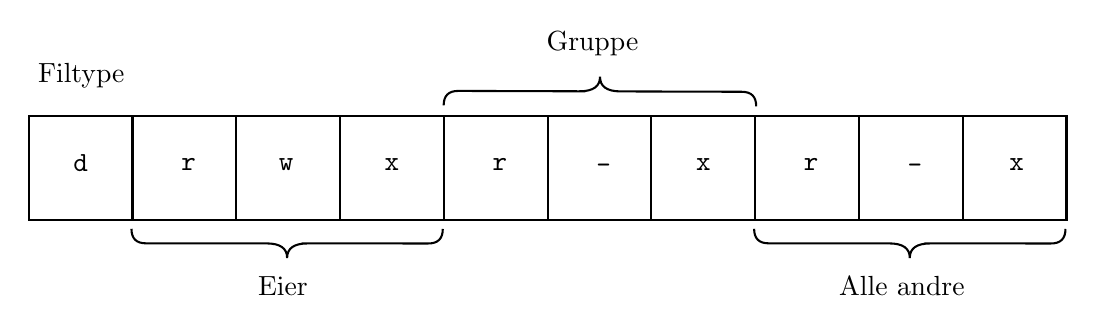
\begin{tikzpicture}[x=0.75pt,y=0.75pt,yscale=-1,xscale=1]
%uncomment if require: \path (0,300); %set diagram left start at 0, and has height of 300

%Shape: Square [id:dp1577110860128721] 
\draw   (100,116) -- (150,116) -- (150,166) -- (100,166) -- cycle ;
%Shape: Square [id:dp1892620238726499] 
\draw   (150,116) -- (200,116) -- (200,166) -- (150,166) -- cycle ;
%Shape: Square [id:dp38131901865551] 
\draw   (200,116) -- (250,116) -- (250,166) -- (200,166) -- cycle ;
%Shape: Square [id:dp01826293318430472] 
\draw   (250,116) -- (300,116) -- (300,166) -- (250,166) -- cycle ;
%Shape: Square [id:dp19897933719983518] 
\draw   (300,116) -- (350,116) -- (350,166) -- (300,166) -- cycle ;
%Shape: Square [id:dp654246426498146] 
\draw   (350,116) -- (400,116) -- (400,166) -- (350,166) -- cycle ;
%Shape: Square [id:dp3647984331806591] 
\draw   (400,116) -- (450,116) -- (450,166) -- (400,166) -- cycle ;
%Shape: Square [id:dp14664904821684455] 
\draw   (450,116) -- (500,116) -- (500,166) -- (450,166) -- cycle ;
%Shape: Square [id:dp8777271275416056] 
\draw   (500,116) -- (550,116) -- (550,166) -- (500,166) -- cycle ;
%Shape: Square [id:dp6186895862983577] 
\draw   (550,116) -- (600,116) -- (600,166) -- (550,166) -- cycle ;
%Shape: Brace [id:dp7579742302595935] 
\draw   (149.5,170.4) .. controls (149.5,175.07) and (151.83,177.4) .. (156.5,177.4) -- (214.5,177.43) .. controls (221.17,177.44) and (224.5,179.77) .. (224.49,184.44) .. controls (224.5,179.77) and (227.83,177.44) .. (234.5,177.44)(231.5,177.44) -- (292.5,177.47) .. controls (297.17,177.48) and (299.5,175.15) .. (299.5,170.48) ;
%Shape: Brace [id:dp5277831906215735] 
\draw   (449.5,170.4) .. controls (449.5,175.07) and (451.83,177.4) .. (456.5,177.4) -- (514.5,177.43) .. controls (521.17,177.44) and (524.5,179.77) .. (524.49,184.44) .. controls (524.5,179.77) and (527.83,177.44) .. (534.5,177.44)(531.5,177.44) -- (592.5,177.47) .. controls (597.17,177.48) and (599.5,175.15) .. (599.5,170.48) ;
%Shape: Brace [id:dp44661745830029576] 
\draw   (450.5,111.4) .. controls (450.51,106.73) and (448.19,104.39) .. (443.52,104.38) -- (385.23,104.21) .. controls (378.56,104.19) and (375.24,101.85) .. (375.25,97.18) .. controls (375.24,101.85) and (371.9,104.17) .. (365.23,104.15)(368.23,104.16) -- (306.94,103.97) .. controls (302.27,103.96) and (299.93,106.28) .. (299.92,110.95) ;

% Text Node
\draw (120,133) node [anchor=north west][inner sep=0.75pt]   [align=left] {\texttt{d}};
% Text Node
\draw (172,135) node [anchor=north west][inner sep=0.75pt]   [align=left] {\texttt{r}};
% Text Node
\draw (219,135) node [anchor=north west][inner sep=0.75pt]   [align=left] {\texttt{w}};
% Text Node
\draw (270,135) node [anchor=north west][inner sep=0.75pt]   [align=left] {\texttt{x}};
% Text Node
\draw (322,135) node [anchor=north west][inner sep=0.75pt]   [align=left] {\texttt{r}};
% Text Node
\draw (372,135) node [anchor=north west][inner sep=0.75pt]   [align=left] {\texttt{-}};
% Text Node
\draw (420,135) node [anchor=north west][inner sep=0.75pt]   [align=left] {\texttt{x}};
% Text Node
\draw (472,135) node [anchor=north west][inner sep=0.75pt]   [align=left] {\texttt{r}};
% Text Node
\draw (522,135) node [anchor=north west][inner sep=0.75pt]   [align=left] {\texttt{-}};
% Text Node
\draw (571,135) node [anchor=north west][inner sep=0.75pt]   [align=left] {\texttt{x}};
% Text Node
\draw (103,89) node [anchor=north west][inner sep=0.75pt]   [align=left] {Filtype};
% Text Node
\draw (209,192) node [anchor=north west][inner sep=0.75pt]   [align=left] {Eier};
% Text Node
\draw (489,192) node [anchor=north west][inner sep=0.75pt]   [align=left] {Alle andre};
% Text Node
\draw (348,74) node [anchor=north west][inner sep=0.75pt]   [align=left] {Gruppe};


\end{tikzpicture}
    \caption{Filegenskaper fra \texttt{ls -l}.}
    \label{fig:2-flagg-ls}
\end{figure}

I eksempelet i figur \ref{fig:2-flagg-ls} kan eieren gjøre hva han eller hun vil, mens gruppen som eier filen og alle andre kan gjøre alt bortsett fra å endre på filen (mangel på \verb|w|). 

Etter denne filbeskrivelsen kommer et tall (\verb|2| i eksempelet). Dette er antall \textit{hardlenker} filen har, og har med hvordan filen er lagret på. Deretter følger navn på eieren av filen (\verb|student| i eksempelet), og gruppen som eier filen (også \verb|student| i eksempelet - disse trenger ikke være like). Tallet \verb|4096| som følger hver linje i eksempelet er antall byte som filen okkuperer - men ettersom mapper egentlig bare er pekere som forteller hvilke filer den inneholder, er dette tallet bare størrelsen på pekeren - altså ikke størrelsen på det mappen inneholder. Til slutt kommer en timestamp av når filen sist ble endret, og navnet på filen.

\cprotect\subsection{\lstinline{cd}}

Kommandoen \verb|cd| er en av de viktigste kommandoene i Linux og blir brukt for å navigere inn- og ut fra mapper. Eksempelvis kaller man \verb|cd Downloads| om man ønsker å bevege seg inn i mappen \verb|Downloads|.

For å bevege seg et nivå opp substituerer man mappenavnet med to punktum: \verb|cd ..|. For eksempel om man er i mappen \verb|Downloads| vil \verb|cd ..| navigere brukeren til hjemmemappen.

I Linux har to punktum blitt definert som foreldremappen, mens ett punktum definerer mappen som brukeren befinner seg i. Dette betyr at kommandoen \verb|cd .| flytter brukeren inn i mappen som man allerede befinner seg i.

Noe annet som også kan være veldig nyttig er \verb|cd -|. \verb|cd -| brukes for å navigere brukeren tilbake til der man sist var. 

\cprotect\subsection{\lstinline{mkdir}}
En nyttig kommando for videre bruk er \verb|mkdir| (\textit{make directory}). Dette er en kommando som brukes for å opprette en mappe. Om man vil opprette en mappe kalt \verb|demo| og bevege seg inn i den kan man eksempelvis
 kalle:

\begin{lstlisting}[mathescape=true]
student@Ubuntu:$\smallsim$$\verb|$|$ mkdir demo
student@Ubuntu:$\smallsim$$\verb|$|$ cd demo
\end{lstlisting}

\cprotect\subsection{\lstinline{touch}}

Kommandoen \verb|touch| angir endrings- og tilgangstider for filer.  Hvis en fil ikke finnes, opprettes den med standardtillatelser. 

\begin{lstlisting}[mathescape=true]
student@Ubuntu:$\smallsim$$\verb|$|$ touch newfile.c
student@Ubuntu:$\smallsim$$\verb|$|$ ls

Documents Downloads Pictures Music
Public Videos Desktop Templates newfile.c
\end{lstlisting}


\cprotect\subsection{\lstinline{file}}

En annen nyttig kommando er \verb|file|. \verb|file| brukes for å skaffe seg informasjon om en fil. For eksempel:

\begin{lstlisting}[mathescape=true]
student@Ubuntu:$\smallsim$$\verb|$|$ file Downloads
Downloads: directory

student@Ubuntu:$\smallsim$$\verb|$|$ file main.c
main.c: C source, ASCII text
\end{lstlisting}



\cprotect\subsection{\lstinline{cat}}

Gitt nå at man har lyst til å ta en titt på innholdet i \verb|main.c| som man allerede vet er en \verb|C|-fil på grunn av kommandoen \verb|file|. Da kan man bruke kommandoen \verb|cat|. \verb|cat| tar innholdet i en fil og skriver det ut i terminalen. For eksempel:

\begin{lstlisting}[mathescape=true]
student@Ubuntu:$\smallsim$$\verb|$|$ cat main.c

#include <stdio.h>

int main(){
    printf("Welcome to TTK4235 - Embedded Systems\n");
    printf("In this course, we will program micro:bits and PLCs.\n");
    printf("Hopefully, you will have fun =).\n");
    return 0;
}
\end{lstlisting}


\cprotect\subsection{\lstinline{man}}

\verb|man|, kort for \textit{manual page} er den viktigste kommandoen i Linux. Denne kommandoen brukes for å lære om bruken av en hvilken som helst kommando. Et relevant eksempel er kommandoen \verb|man ls| som brukes for å generere en liste over hvilke flagg som \verb|ls| støtter. 

I tillegg er det også mulig å kalle \verb|man man| for å få enda mer informasjon om hvordan man kan bruke \verb|man|. Dersom dette blir gjort, kan man se at \verb|man| grupperer manualene i 9 kategorier - hvor kategori 3 er bibliotekkall. 

Disse kategoriene kan brukes for å spesifisere hvilke kommandoer man vil ha mer informasjon om, dersom det er flere programmer eller bibliotekkall med samme navn. For eksempel har man programmet \verb|printf|, som  man kan få informasjon om ved å kalle \verb|man printf|. Om man derimot vil ha dokumentasjon på funksjonen med samme navn i \verb|C|, kan man kalle \verb|man 3 printf|.

\cprotect\subsection{\lstinline{sudo}}

Som vanlig bruker kan man ikke bruke alle kommandoer. Noen kommandoer er forbeholdt brukere med ekstra rettigheter (\textit{root}). Om man får \verb|permission denied| når man kaller en kommando, kan man midlertidig eskalere brukerrettighetene til \textit{root}-rettigheter ved å kalle kommandoen med \verb|sudo| foran (kort for \textbf{s}uper\textbf{u}ser \textbf{do}). 

\cprotect\subsection{\lstinline{apt}}

Til slutt er det verdt å vite hvordan man installerer nye programmer og pakker. De fleste Linux-distribusjoner bruker en pakkemanager for å håndtere installerte programmer. På denne måten har man en sentralisert løsning for å installere og oppdatere programvarer. 

I Ubuntu bruker man \verb|apt| som pakkemanager. For eksempel kan man installere programmeringsspråket \verb|Ruby| sin interpreter ved å kalle \verb|sudo apt install ruby|. Informasjon om hva programvaren \verb|ruby| inneholder kan fås ved å kalle \verb|apt show ruby|.

For å oppdatere alle installerte programvarer til nyeste versjon som Ubuntu har tilgjengelig kaller man \verb|sudo apt update|, etterfulgt av \verb|sudo apt upgrade|. Kommandoen \verb|update| oppdaterer listen over tilgjengelig programvarer som kan oppdateres, mens kommandoen \verb|upgrade| installerer de nyeste oppdateringene. For mer informasjon om hvilke kommandoer \verb|apt| støtter kan man kalle \verb|man apt|.

En ting som er verdt å vite om er at Ubuntu tester ut nye pakker en stund før de legges til oversikten som \verb|apt| har tilgang til. Med andre ord kan det ta en stund før nyeste versjon av programvare kommer til Ubuntu. 




\cprotect\subsection{\lstinline{nano}}
Når man jobber med GNU/Linux er det ikke alltid gitt at man kan bruke tekstredigeringsprogrammer som \textit{Word}, \textit{Visual Studio Code} eller \textit{Notepad++}. Derfor er det lurt å kunne bruke verktøy som fungerer \textit{uten} et grafisk brukergrensesnitt. \verb|nano|, kort for \textit{\textbf{N}ano's \textbf{ANO}ther Editor}, er et enkelt tekstredigeringsvektøy som fungerer i terminalen. 

\begin{lstlisting}[mathescape=true]
student@Ubuntu:$\smallsim$$\verb|$|$ nano main.c
\end{lstlisting}

Nederst i terminalvinduet vil du se enkelte kommandoforslag som \verb|^X| for \textit{Exit}. Kontraintuitivt betyr \verb|^| at vi skal bruke \verb|Ctrl|. Dette betyr at for å gå ut av \verb|nano| må vi taste \verb|Ctrl| og \verb|X| etter hverandre. For å forkaste eller lagre endringene du har gjort i en fil må du deretter taste \verb|Y| for "Yes" og \verb|N| for "No".

\cprotect\subsection{Kommentar til Tekstredigering}

Det finnes veldig mange populære programmer for tekst- og filredigering for GNU/Linux. Noen av dem er \verb|vim|, \verb|neovim|, \verb|emacs|, \verb|gedit|, \verb|sublime-text|, \verb|notepadqq|, \verb|VSCode|\footnote{Kort for \textit{Visual Studio Code}, laget av Microsoft} og \verb|nano|. Disse varierer både i grensesnitt og brukervennlighet. For små endringer i filer kan alternativ som \verb|nano| og \verb|vim| være gode programmer. Dersom du ikke har noe tidligere erfaring med GNU/Linux anbefaler vi at du bruker enten \href{https://code.visualstudio.com/}{VSCode} eller open-source programmet \href{https://github.com/VSCodium/vscodium}{VSCodium}\footnote{VSCode er basert på VSCodium} for mer omfattende endringer. Disse programmene er \textit{source-code editors} skreddersydde for programvareutvikling. Videre i øvingsopplegget kommer vi til å bruke \verb|VSCode| som eksemel på hvordan vi kan bruke verktøyene vi lærer om i et utviklingsmiljø.

\end{alphasection}
\setcounter{section}{0}

